\documentclass[11pt]{article}
\usepackage{notes}
\definecolor{AccN}{HTML}{9B5E1A}
\begin{document}
\titlepg{8}{Reinforcement Learning Part 3:\\Multi-Agent Systems and Autonomous Platforms}{Dec-POMDPs, centralised training with decentralised execution, VDN, QMIX, MAPPO, MADDPG, credit assignment, emergent communication, and the ethics of autonomy}
\tableofcontents
\newpage

\section{From One Agent to a Team}
Military operations are team efforts: infantry, armour, artillery, reconnaissance drones and aircraft act simultaneously, each seeing only part of the battlefield, toward a shared objective, against an adversary that adapts. Single-agent RL cannot represent this directly: one agent controls one entity, observes one viewpoint and receives credit for its own actions. \textbf{Multi-agent reinforcement learning} (MARL) trains several agents that learn concurrently in a shared environment.

\textbf{Case study.} A combined-arms team of six agents --- infantry, armour, artillery, two ISR drones and one SEAD aircraft --- must destroy a defended position held by two surface-to-air missile (SAM) sites and four OPFOR infantry units. Each agent observes 42 features (its own position, health, ammunition and role; units within its sensor range; friendly positions when communications are not jammed).

\section{Formalising the Problem}
\begin{definition}{decentralised POMDP}
A Dec-POMDP is $(S,\{A_i\}_{i=1}^N,P,r,\{\Omega_i\},O,\gamma)$: global state $s$; each agent $i$ has actions $A_i$ and receives a private observation $o_i\in\Omega_i$ generated by $O$; the joint action $\mathbf a=(a_1,\ldots,a_N)$ drives the transition $P(s'|s,\mathbf a)$; in cooperative settings all agents share the reward $r(s,\mathbf a)$. Each agent acts with its own policy $\pi_i(a_i\mid o_i)$ (or its observation history).
\end{definition}
\textbf{Settings.} \emph{Fully cooperative} (shared reward: a combined-arms attack); \emph{fully competitive} (zero-sum: Blue vs Red); \emph{mixed} (a cooperating Blue team against a cooperating Red team) --- the usual military case.

\subsection{The core difficulties}
\begin{itemize}
\item \textbf{Non-stationarity.} From agent $i$'s viewpoint the other agents are part of the environment, and they are learning; the environment it faces keeps changing, so single-agent convergence guarantees no longer hold.
\item \textbf{Partial observability.} No unit sees the whole battlefield.
\item \textbf{Credit assignment.} A shared reward does not say which agent's actions produced it.
\item \textbf{Scalability.} The joint action space grows exponentially: six agents with 10 actions each have $10^6$ joint actions.
\item \textbf{Coordination.} Good joint actions may require agents to act in complementary ways (suppress, then advance).
\end{itemize}

\section{Centralised Training, Decentralised Execution}
\begin{definition}{CTDE}
During \emph{training} (in simulation) learning algorithms may use global information --- the full state, all observations and all actions --- for example in a centralised critic or mixing network. At \emph{execution} each agent acts on its own local observation with its own policy; the centralised components are discarded.
\end{definition}
CTDE mirrors \textbf{mission command}: commanders rehearse a plan with full shared intelligence, then units execute under radio silence using local initiative. Because coordination is encoded in the trained policies, the system needs no communication during execution and is resilient to jamming.
\begin{center}\begin{tikzpicture}
\begin{scope}\node[font=\small\bfseries,AccN]at(2.1,2.1){training};\node[nd,fill=NavyN,text=white,minimum width=4cm](c)at(2.1,1.3){central critic / mixer: sees $s$};\foreach \i in {1,2,3}{\node[nd,fill=AccN!15](a\i)at(\i*1.4-0.7,0){actor \i};\draw[arr,<->](a\i)--(c);}\end{scope}
\draw[-{Stealth},thick,AccN](4.9,0.6)--(6.4,0.6)node[midway,above,font=\scriptsize]{deploy actors};
\begin{scope}[xshift=7cm]\node[font=\small\bfseries,AccN]at(2.1,2.1){execution};\foreach \i in {1,2,3}{\node[nd,fill=AccN!15](b\i)at(\i*1.4-0.7,0){actor \i};\node[nd,font=\scriptsize](o\i)at(\i*1.4-0.7,1.1){$o_\i$};\draw[arr](o\i)--(b\i);}\end{scope}
\end{tikzpicture}\\{\small\color{GreyN}Figure 1: CTDE --- centralised information during training only.}\end{center}

\subsection{The naive baseline: independent learners}
Independent Q-learning (IQL) trains each agent as if the others were part of the environment. It is simple and scales, but ignores non-stationarity and coordination: 58.3\% mission success in the case study --- the floor against which the CTDE methods are judged.

\section{Value Decomposition: VDN and QMIX}
\subsection{The individual--global--max property}
We want a joint value $Q_{\text{tot}}(s,\mathbf a)$ for training, but decentralised greedy action selection at execution. These are consistent if
\[\arg\max_{\mathbf a}Q_{\text{tot}}(s,\mathbf a)=\Big(\arg\max_{a_1}Q_1(o_1,a_1),\ldots,\arg\max_{a_N}Q_N(o_N,a_N)\Big),\]
the \textbf{individual--global--max (IGM)} property.

\subsection{VDN}
Value decomposition networks (Sunehag et al., 2018) set $Q_{\text{tot}}=\sum_iQ_i$. IGM holds trivially, since the sum is maximised by maximising each term, but additivity cannot represent situations whose value depends non-linearly on the state.

\subsection{QMIX}
QMIX (Rashid et al., 2018) mixes the individual values non-linearly, $Q_{\text{tot}}=f(Q_1,\ldots,Q_N;s)$, under the constraint
\[\frac{\partial Q_{\text{tot}}}{\partial Q_i}\ge0\quad\forall i.\]
\begin{derivation}{monotonicity implies IGM}
Suppose $\mathbf a^*$ maximises $Q_{\text{tot}}$ but agent $j$'s component $a_j^*$ is not $\arg\max Q_j$. Replace it by $\arg\max Q_j$, keeping the others fixed: $Q_j$ does not decrease, and because $Q_{\text{tot}}$ is non-decreasing in every $Q_i$, $Q_{\text{tot}}$ does not decrease. Repeating for each agent yields the tuple of individual maxima with $Q_{\text{tot}}$ at least as large, so it is also a maximiser. Each agent can therefore act greedily on its own $Q_i$ with no negotiation.
\end{derivation}
\textbf{Architecture.} Each agent has a recurrent network (GRU, to cope with partial observability) producing $Q_i(o_i,\cdot)$; a mixing network combines them with weights generated by \textbf{hypernetworks} from the global state $s$, made non-negative by taking absolute values (biases may be any sign). Training minimises the TD error of $Q_{\text{tot}}$ with replay and target networks.
\begin{pitfall}{what monotonic mixing cannot represent}
If one agent's best action depends on another's choice (``advance only if the other unit holds''), the joint value is not monotonic in the individual values. QMIX then learns a compromise; methods with richer factorisations or communication are needed.
\end{pitfall}
\textbf{Case result:} 74.1\% success, 1.8 friendly casualties per mission, 38.2 turns; the SEAD aircraft learned to neutralise SAM sites first, with ground units advancing only afterwards --- textbook suppression-of-enemy-air-defences doctrine, discovered from reward alone.

\section{Policy-Gradient MARL: MAPPO and MADDPG}
\subsection{MAPPO}
Multi-agent PPO (Yu et al., 2022) uses (1) a \textbf{shared actor} $\pi(a_i|o_i,\text{id}_i;\theta)$ for all agents, with a one-hot agent identifier so roles can differ; (2) a \textbf{centralised critic} $V(s;\phi)$ on the global state; (3) PPO clipping per agent, $L=\frac1N\sum_iL_i^{\text{CLIP}}$; (4) advantage normalisation across agents and steps. Parameter sharing means every agent's experience trains the same network, greatly improving sample efficiency for similar agents. Case result: \textbf{82.4\%} success, 1.2 casualties, 33.7 turns --- against \textbf{81.3\%} for a team of three experienced human planners.
\begin{pitfall}{is 82.4\% really better than 81.3\%?}
A 1.1-point gap from a single evaluation, without the number of episodes or a confidence interval, cannot establish superiority (Lecture~1). With, say, 300 evaluation episodes the standard error of each rate is about 2.2 points; the honest statement is ``comparable to expert planners in this simulation''.
\end{pitfall}

\subsection{MADDPG}
MADDPG (Lowe et al., 2017) gives each agent a deterministic actor $\mu_i(o_i)$ and its own centralised critic $Q_i(s,a_1,\ldots,a_N)$, which sees every agent's action. Because critics condition on others' actions, the environment is stationary from the critic's viewpoint, and agents can have different rewards --- suitable for continuous actions and mixed cooperative--competitive games. Case result: 79.2\%.

\section{Credit Assignment and COMA}
With a shared reward of $+100$, a naive equal split gives $+16.7$ to every agent --- including an artillery unit whose shot missed and a drone that malfunctioned. Agents then learn that idleness is rewarded: the \textbf{free-rider} problem. Counterfactual multi-agent policy gradients (COMA; Foerster et al., 2018) ask: how much better was agent $i$'s actual action than what it would have done on average, with everyone else's actions fixed?
\[b_i(s,\mathbf a_{-i})=\sum_{a_i'}\pi_i(a_i'|o_i)\,Q\big(s,(a_i',\mathbf a_{-i})\big),\qquad A_i(s,\mathbf a)=Q(s,\mathbf a)-b_i(s,\mathbf a_{-i}).\]
\begin{example}{a counterfactual advantage}
For the artillery agent, the centralised critic estimates $Q=62$ for the actual joint action (artillery fired early). Holding the other five actions fixed, the critic's values for artillery's alternatives are fire-early 62, fire-on-cue 70, hold 66, with policy probabilities 0.5, 0.3, 0.2. Baseline $b=0.5(62)+0.3(70)+0.2(66)=65.2$; advantage $A=62-65.2=-3.2$: the early shot is discouraged even though the team succeeded.
\end{example}
In the case study the counterfactual advantages were infantry $+8.4$, armour $+12.1$, artillery $-3.2$, ISR drone 1 $+9.8$, ISR drone 2 $-1.1$, SEAD $+11.4$: the unhelpful agents are penalised and the critical ones credited.
\begin{pitfall}{a claim to check}
The source slides state that these advantages sum to approximately zero ``as a baseline property''. They sum to $+37.4$. Counterfactual advantages have zero mean over each agent's \emph{own} action distribution, not across agents.
\end{pitfall}

\section{Emergent Communication and Tactics}
Adding a learned message channel (each agent broadcasts an 8-dimensional vector and receives the others') lets agents invent a code by gradient descent. Linear probes showed message dimensions encoding enemy positions seen by the drones, SAM lock-on status, and fuel state. CommsMAPPO reached \textbf{88.1\%} success, 0.9 casualties, 29.4 turns. Learned codes are opaque to humans and could be spoofed; they must be decoded, monitored and secured.

Replays revealed tactics never explicitly rewarded: SEAD-first in 100\% of episodes; ISR drones taking high-ground overwatch positions (88\%); infantry fixing the enemy frontally while armour flanked (71\% of successful episodes); artillery fire timed to the flanking move (67\%); and bounding advance. MARL rediscovers valid doctrine and can suggest new coordination patterns --- but it also finds degenerate ones: in some runs agents learned to conserve ammunition by \emph{not firing}, locally rational under the reward and tactically absurd.

\section{Results Summary}
\begin{center}\small\renewcommand{\arraystretch}{1.2}
\begin{tabular}{llcccc}\toprule Method & Type & Success & Casualties & Turns & Training episodes\\\midrule IQL & independent & 58.3\% & 2.8 & 44.1 & 100K\\ QMIX & value CTDE & 74.1\% & 1.8 & 38.2 & 200K\\ MADDPG & actor--critic CTDE & 79.2\% & 1.6 & 35.8 & 250K\\ MAPPO & PG CTDE & 82.4\% & 1.2 & 33.7 & 150K\\ \textbf{CommsMAPPO} & PG + comms & \textbf{88.1\%} & \textbf{0.9} & \textbf{29.4} & 180K\\ Human experts & --- & 81.3\% & 1.6 & 41.8 & ---\\\bottomrule\end{tabular}\end{center}
Choice of method: MAPPO as a robust default for cooperative teams; QMIX for cooperative discrete tasks where off-policy data reuse and interpretable per-agent values matter; MADDPG for continuous actions and mixed settings; add learned communication only where channels are available and secure.

\section{Autonomy, Law and Ethics}
\subsection{Levels of autonomy}
\begin{center}\small\renewcommand{\arraystretch}{1.25}
\begin{tabularx}{\textwidth}{>{\bfseries}lX}\toprule Level 1 & Human-operated; AI assists (e.g.\ target cueing).\\ Level 2 & Human-on-the-loop: AI nominates actions, a human approves each one --- the advisory mode advocated in this course.\\ Level 3 & AI engages without per-action approval within set criteria; contested under international humanitarian law (IHL).\\ Level 4 & Fully autonomous for extended missions; prohibited in most militaries.\\\bottomrule\end{tabularx}\end{center}

\subsection{Manned--unmanned teaming}
A pilot directs several unmanned wingmen running trained MARL policies: the human sets objectives, threat priorities and rules of engagement (ROE); the agents optimise within them. ROE can be encoded as penalties (for engaging non-combatants or disproportionate force), but a penalty only makes violations less likely --- it is not a legal safeguard. Open challenges: calibrating human trust, adversarial exploitation of learned patterns, accountability for AI-advised actions, and transfer from simulation (an 82\% simulated success may correspond to around 65\% in reality).

\subsection{The bright line}
IHL requires distinction (combatants vs civilians), proportionality (expected civilian harm not excessive relative to military advantage) and precautions in attack. These are contextual legal judgements that no reward function can encode. This course therefore treats MARL as decision support: \textbf{the human remains the decision-maker for lethal force}, with a full audit trail from sensor input to AI recommendation to human decision to outcome.

\section{Deeper Dive I: Game-Theoretic Foundations}
\subsection{Games, best responses and equilibria}
A \textbf{normal-form game} lists each player's actions and the payoffs of every combination. A \textbf{best response} is an action that maximises a player's payoff given the others' choices. A \textbf{Nash equilibrium} is a profile in which every player is best-responding, so no one gains by deviating alone. In two-player \textbf{zero-sum} games (one side's gain is the other's loss), von Neumann's minimax theorem guarantees an equilibrium value, possibly requiring \emph{mixed} (randomised) strategies.
\begin{example}{where to attack, where to defend}
Blue attacks North (AN) or South (AS); Red defends North (DN) or South (DS). Payoffs to Blue (Red receives the negative):
\begin{center}\renewcommand{\arraystretch}{1.25}\begin{tabular}{lcc}\toprule & Red DN & Red DS\\\midrule Blue AN & $-1$ & $+3$\\ Blue AS & $+2$ & $-2$\\\bottomrule\end{tabular}\end{center}
No pure profile is stable: whatever Blue does, Red wants to defend there, and vice versa. Blue chooses $P(\text{AN})=p$ to make Red indifferent: $-p+2(1-p)=3p-2(1-p)\Rightarrow2-3p=5p-2\Rightarrow p=0.5$. Red chooses $P(\text{DN})=q$ to make Blue indifferent: $-q+3(1-q)=2q-2(1-q)\Rightarrow3-4q=4q-2\Rightarrow q=0.625$. The game value is $0.5(-1)+0.5(2)=+0.5$ to Blue.
\end{example}
\begin{keypoint}In adversarial settings the optimal policy is often \emph{randomised}: a predictable attacker is defeated. This is the game-theoretic reason for SAC's entropy, for deception, and for evaluating learned policies against adaptive opponents rather than fixed scripts.\end{keypoint}

\subsection{Self-play, fictitious play and leagues}
Training an agent against copies of itself (\textbf{self-play}) can cycle --- rock beats scissors beats paper --- rather than converge. \textbf{Fictitious play} best-responds to the \emph{average} of past opponents and converges in two-player zero-sum games. \textbf{League training} (as in AlphaStar) maintains a population of past and specialised ``exploiter'' agents so that the main agent is robust to many strategies, not just its latest self.

\section{Deeper Dive II: QMIX Mixing by Hand}
\begin{example}{a one-hidden-unit mixer}
Agents report $Q_1=2$, $Q_2=5$. From the global state, the hypernetworks produce raw weights $(0.5,-1.2)$, bias $b_1=-1$, output weight $-0.8$ and bias $b_2=2$. Taking absolute values of the weights: hidden $h=\text{ELU}(0.5\times2+1.2\times5-1)=\text{ELU}(6)=6$; $Q_{\text{tot}}=0.8\times6+2=6.8$. If agent 2's value rises to 6, $h=7.2$ and $Q_{\text{tot}}=7.76$: an individual improvement can only raise the team value, which is exactly the monotonicity that makes decentralised greedy action selection consistent.
\end{example}
\begin{center}\begin{tikzpicture}
\foreach \i in {1,2,3}{\node[nd,fill=AccN!15](q\i)at(\i*2-2,0){agent \i\\GRU $\to Q_\i$};}
\node[nd,fill=NavyN,text=white,minimum width=5cm](mx)at(2,1.7){mixer: $Q_{\text{tot}}=f(Q_1,Q_2,Q_3)$};
\foreach \i in {1,2,3}{\draw[arr](q\i)--(mx);}
\node[nd,fill=AmbN!25](h)at(7,1.7){hypernetworks\\$s\to|W|,b$};\draw[arr](h)--(mx);\node[nd](s)at(7,0){global state $s$};\draw[arr](s)--(h);
\end{tikzpicture}\\{\small\color{GreyN}Figure 2: QMIX architecture. Weights generated from the state are made non-negative.}\end{center}

\section{Deeper Dive III: MAPPO in Practice}
\begin{center}\begin{minipage}{0.92\textwidth}\small\ttfamily
for iteration:\\
\hspace*{1em}roll out shared actor pi(a\_i | o\_i, id\_i) for all agents in parallel envs\\
\hspace*{1em}critic input: global state s (or concatenated observations) + agent id\\
\hspace*{1em}advantages: GAE per agent from V(s); normalise across agents and steps\\
\hspace*{1em}value targets: normalise (running mean/std) for stable critic training\\
\hspace*{1em}K epochs of clipped PPO updates on actor and critic (eps about 0.2)
\end{minipage}\end{center}
Practical findings (Yu et al., 2022): MAPPO is competitive with or better than off-policy methods on cooperative benchmarks when value normalisation, agent-specific global-state inputs and modest numbers of PPO epochs are used; parameter sharing works well for homogeneous agents, while heterogeneous teams may use separate actors per role.

\section{Deeper Dive IV: Learning to Communicate}
Differentiable communication (CommNet, DIAL) lets gradients flow from the team objective back through received messages into senders, so agents learn \emph{what} to say. Robustness matters operationally: train with random message dropout and noise so policies degrade gracefully under jamming; limit bandwidth (few dimensions, discretised tokens); and test whether policies still function with the channel removed. Learned codes should be audited with probes and treated as security-relevant: an adversary who learns the code could inject false messages.

\section{Deeper Dive V: Rules of Engagement as Constraints}
Encoding ROE as reward penalties lets the optimiser trade violations against mission reward. \textbf{Constrained MDPs} instead maximise $\mathbb E[R]$ subject to $\mathbb E[C]\le d$ for a cost $C$ (e.g.\ engagements of non-combatant tracks). The Lagrangian $L=\mathbb E[R]-\lambda(\mathbb E[C]-d)$ is optimised with $\lambda$ increased whenever the constraint is violated (dual ascent), so the penalty grows until the constraint holds on average. For hard constraints, a \textbf{shield} --- a verified rule-based layer --- blocks prohibited actions before they reach actuators. Neither replaces human legal judgement on distinction and proportionality, but both reduce the space of things a human must catch.

\section{Deeper Dive VI: Evaluating Multi-Agent Systems}
Evaluate against diverse opponents (scripted doctrines, past checkpoints, exploiters, humans); measure \textbf{exploitability} --- how much a best-responding adversary trained against the frozen policy can gain; use \textbf{cross-play} (pair agents trained separately) to test whether coordination relies on brittle private conventions; report means and confidence intervals over seeds and scenarios; and ablate communication to see what breaks when the channel is denied.

\begin{center}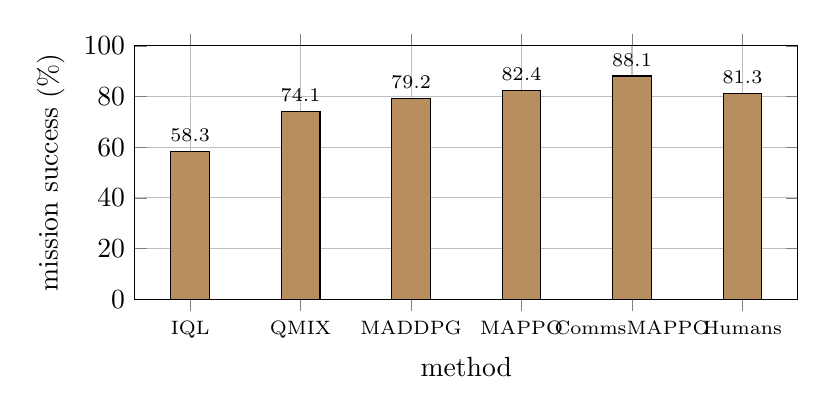
\begin{tikzpicture}\begin{axis}[width=10cm,height=4.8cm,xlabel={method},ylabel={mission success (\%)},ybar,bar width=14pt,symbolic x coords={IQL,QMIX,MADDPG,MAPPO,CommsMAPPO,Humans},xtick=data,x tick label style={font=\scriptsize},ymin=0,ymax=100,nodes near coords,nodes near coords style={font=\scriptsize},grid=major]
\addplot[fill=AccN!70]coordinates{(IQL,58.3)(QMIX,74.1)(MADDPG,79.2)(MAPPO,82.4)(CommsMAPPO,88.1)(Humans,81.3)};
\end{axis}\end{tikzpicture}\\{\small\color{GreyN}Figure 3: combined-arms results (single study, no confidence intervals reported).}\end{center}

\clearpage
\part*{Part C --- Further Theory, Methods and Applications}
\addcontentsline{toc}{part}{Part C --- Further Theory, Methods and Applications}

\section{Markov Games: the Formal Setting}
A \textbf{Markov (stochastic) game} with $n$ agents is a tuple $(S,\{A_i\},P,\{R_i\},\gamma)$: at each step every agent $i$ chooses $a_i$; the joint action $\mathbf a=(a_1,\ldots,a_n)$ determines the next state through $P(s'\mid s,\mathbf a)$ and each agent's reward through $R_i(s,\mathbf a)$. Three cases organise the field:
\begin{itemize}
\item \textbf{Fully cooperative} --- all agents share one reward (the Blue team of Lecture~8). The problem is a single MDP over joint actions in principle, but its action space grows exponentially and execution must be decentralised.
\item \textbf{Zero-sum} --- two sides with $R_1=-R_2$ (Blue versus Red). Each side should maximise its worst-case return; the solution concept is the \textbf{minimax} equilibrium, and minimax-Q learning replaces Q-learning's max by the value of a matrix game at each state.
\item \textbf{General-sum} --- coalition partners with overlapping but different interests. Solution concepts include Nash and correlated equilibria, and there may be many equilibria of very different quality.
\end{itemize}
When agents see only local observations, the cooperative case becomes the Dec-POMDP of the main text, and even finding the optimal joint policy for a finite horizon is NEXP-complete --- formal confirmation that decentralised coordination is fundamentally hard, and that CTDE methods are approximations.

\section{Security Games: Commit, Then Be Observed}
In many defence settings the defender acts first and the attacker observes before choosing: patrol schedules, checkpoint locations, air-defence coverage. This is a \textbf{Stackelberg game}. The defender commits to a \emph{randomised} allocation; the attacker, having watched long enough to learn the probabilities, attacks the target that is best for them.
\begin{example}{covering two targets with one patrol}
Target~1 (a fuel depot) and target~2 (a bridge). If the attacker strikes an uncovered target their payoff is 10 or 6 respectively; if covered, $-5$ or $-3$. The defender loses 10 or 6 at an uncovered target and gains 5 or 3 at a covered one. The defender covers target~1 with probability $c$ and target~2 with $1-c$.\\[2pt]
\textbf{Naive 50/50 patrol:} the attacker's expected payoffs are $0.5(-5)+0.5(10)=2.5$ at target~1 and $1.5$ at target~2, so they hit target~1, and the defender's expected payoff is $-2.5$.\\
\textbf{Optimal commitment:} make the attacker indifferent between targets: $10-15c=6-9(1-c)\Rightarrow c=13/24=0.54$. Both targets then offer the attacker 1.875, and the defender's expected payoff improves to $-1.875$. Covering the more valuable target slightly more than half the time --- and doing so \emph{unpredictably} --- beats both even and deterministic patrols.
\end{example}
\begin{center}\begin{tikzpicture}\begin{axis}[width=7.6cm,height=4.6cm,xmin=0,xmax=1,ymin=-6,ymax=11,xlabel={coverage of target 1, $c$},ylabel={attacker payoff},grid=both,grid style={GreyN!15},font=\scriptsize,legend style={font=\tiny,at={(0.98,0.98)},anchor=north east}]
\addplot[RedN,thick,domain=0:1]{10-15*x};\addlegendentry{attack target 1}
\addplot[BluN,thick,domain=0:1]{-3+9*x};\addlegendentry{attack target 2}
\addplot[only marks,mark=*,AccN]coordinates{(0.5417,1.875)};
\draw[dashed,GreyN](axis cs:0.5417,-6)--(axis cs:0.5417,1.875);\node[font=\tiny,anchor=north west]at(axis cs:0.55,1.6){$c^*=0.54$};
\end{axis}\end{tikzpicture}\\*{\small\color{GreyN}Figure C1: the attacker takes the higher line; the defender's best commitment is where the lines cross.}\end{center}

Security games have been fielded for real scheduling problems, for example randomised checkpoint and patrol schedules at Los Angeles International Airport (ARMOR) and for US Coast Guard patrols (PROTECT). The lesson for learning agents: a predictable policy is an exploitable policy, and in adversarial settings the right answer is often a probability distribution, not a single best action.

\section{Learning in Games: Fictitious Play, Self-Play and Leagues}
\subsection{Fictitious play}
Each player assumes the opponent plays according to the empirical frequencies of their past actions and best-responds to that mixture.
\begin{example}{fictitious play on matching pennies}
Row wins if the two coins match; column wins if they differ. Starting from (heads, heads), the empirical frequency of row playing heads runs 1.00, 1.00, 0.75, 0.60, 0.50, 0.43, 0.38, 0.33 over the first eight rounds, while column's swings 0.50, 0.33, 0.25, 0.20, 0.17, 0.29, 0.38, 0.44. The \emph{play} cycles, but the \emph{frequencies} spiral in toward the equilibrium of 50/50 --- in two-player zero-sum games fictitious play's averages always converge to equilibrium.
\end{example}
\subsection{Self-play and its failure mode}
Training an agent against copies of itself produced superhuman Go and chess play. In games with non-transitive strategies (rock beats scissors beats paper beats rock), naive self-play can chase its own tail: the agent learns to beat its latest self and forgets how to beat older strategies. \textbf{Population-based training} keeps a pool of past and diverse opponents; \textbf{PSRO} (policy-space response oracles) repeatedly adds a best response to a mixture over the population; AlphaStar's \textbf{league} added dedicated ``exploiter'' agents whose only job was to find weaknesses in the main agents. For wargaming the message is clear: an AI opponent is only as robust as the variety of opponents it trained against.
\subsection{Exploitability}
The \textbf{exploitability} of a policy is how much a best-responding opponent could gain against it. Win rate against a fixed opponent can be high while exploitability is also high. Estimating exploitability --- training a fresh adversary specifically against the frozen policy --- is the most informative robustness test for any game-playing agent.

\section{Where Value Factorisation Breaks}
\subsection{A coordination game that VDN and QMIX cannot represent}
Two agents each choose one of three actions; the team reward is
\[R=\begin{pmatrix}8&-12&-12\\-12&0&0\\-12&0&0\end{pmatrix}.\]
The optimum is for both to choose action~1 (reward 8), but if only one of them does, the team is heavily punished.
\begin{example}{VDN's best additive fit}
Fitting $R(a_1,a_2)\approx Q_1(a_1)+Q_2(a_2)$ by least squares over all nine joint actions gives $Q_1=Q_2=(-3.11,\,-1.78,\,-1.78)$. Each agent's greedy action is therefore action~2 or~3, and the team settles on a joint action worth 0 instead of 8. The additive (and, in this case, the monotonic) structure averages away the narrow peak: from either agent's individual viewpoint, action~1 is usually disastrous because the partner usually does something else.
\end{example}
\subsection{Richer factorisations}
\textbf{QTRAN} and \textbf{QPLEX} enlarge the class of representable joint values while preserving the individual-greedy-max (IGM) property, at the cost of harder optimisation; \textbf{weighted QMIX} up-weights the joint actions that matter most (those near the optimum) in the training loss. In practice, coordination problems with sharp, narrow optima are where communication, centralised critics (MAPPO) or explicit coordination protocols earn their keep.

\section{Credit Assignment Beyond COMA}
\subsection{Difference rewards}
Give each agent the change in team reward attributable to it: $D_i=G(\mathbf a)-G(\mathbf a_{-i}\cup c_i)$, where $c_i$ is a default action (often ``do nothing'').
\begin{example}{who mattered in the assault?}
The team reward for a successful assault is 100. Re-simulating with each agent replaced by an idle default gives 40 without the tank, 95 without the drone and 70 without the artillery. Difference rewards: tank 60, artillery 30, drone 5. The tank was decisive; the drone barely contributed this time. Each agent's learning signal now reflects its own effect, which removes the free-rider problem --- at the price of the extra counterfactual simulations (or a learned model of $G$), which COMA's critic provides without re-simulation.
\end{example}
\subsection{Shapley credit}
Difference rewards consider removing one agent at a time; when agents' contributions interact (the drone matters only if the artillery fires), Shapley values average each agent's marginal contribution over all orders of arrival (as in the Lecture~2 text) and divide the team reward fairly. They are expensive to compute exactly but can be approximated by sampling, and they are increasingly used to explain team behaviour after the fact.

\section{Communication, Scale and Other Minds}
\subsection{Learning what to say and to whom}
Differentiable communication (DIAL, CommNet) lets gradients flow through messages so that agents learn what to send. Attention-based schemes (TarMAC) let each agent decide whom to listen to, which matters when bandwidth is scarce. Military communication is contested: training with random message drop-outs, delays and adversarial noise produces policies that degrade gracefully when links are jammed, and penalising message length keeps traffic within emission-control limits.
\subsection{Mean-field reinforcement learning}
For swarms of hundreds of drones, each agent cannot model every other. \textbf{Mean-field RL} approximates the effect of all neighbours by their average action: each agent learns $Q(s,a_i,\bar a_{-i})$, where $\bar a_{-i}$ is the mean action in its neighbourhood. The many-body problem becomes a two-body problem between an agent and the ``field'' of its neighbours, and the method scales to very large populations.
\subsection{Modelling the opponent}
Agents can maintain explicit models of others: predicting their next actions, inferring their goals, or reasoning recursively in \textbf{level-$k$} fashion (``a level-1 agent best-responds to a naive opponent; a level-2 agent best-responds to a level-1 agent''). Recursive reasoning is the formal heart of deception and counter-deception --- and a warning: an agent trained against a modelled opponent is only as good as the model.
\subsection{Teaming with humans}
An agent that coordinates perfectly with copies of itself may coordinate badly with people, because it has learned arbitrary conventions (``always go left first'') that a human partner does not share. \textbf{Zero-shot coordination} methods (for example \emph{other-play}, which trains with randomly relabelled symmetric actions) push agents toward conventions any sensible partner could follow. For manned--unmanned teaming, predictability and legibility --- behaving in ways the human can anticipate and understand --- are as important as raw performance, and trust must be calibrated: neither over-trusting an agent outside its competence nor ignoring it inside.

\section{Evaluating Agents That Play Against Each Other}
\subsection{Elo ratings}
The expected score of player $A$ against player $B$ is $E_A=1/\big(1+10^{(R_B-R_A)/400}\big)$; after a game with result $S_A\in\{0,\tfrac12,1\}$, $R_A\leftarrow R_A+K(S_A-E_A)$.
\begin{example}{rating two agents}
Agent A (1600) plays agent B (1450): $E_A=0.70$. If A loses, with $K=32$ A drops to 1577.5 and B rises to 1472.5. A 150-point gap therefore means A is expected to score about 70\%. Elo assumes strength is one-dimensional; with non-transitive strategies (A beats B, B beats C, C beats A) a single rating misleads, and a full \textbf{cross-play matrix} of results between all agents, together with exploitability, should be reported.
\end{example}
\subsection{What to report}
For multi-agent results in defence studies: win rates and key outcome measures over many seeds with confidence intervals; performance against scripted doctrine, earlier versions, independently trained agents and humans; exploitability by a fresh adversary; behaviour under communication loss and sensor degradation; and expert review of the tactics that emerged, including whether they would be lawful and acceptable.

\section{Law, Policy and Assurance of Autonomous Systems}
\subsection{The legal baseline}
International humanitarian law applies to every weapon, however autonomous: \textbf{distinction} (only military objectives may be attacked), \textbf{proportionality} (expected civilian harm must not be excessive in relation to the anticipated military advantage) and \textbf{precautions in attack}. Article~36 of Additional Protocol~I (1977) requires states party to review new weapons, means and methods of warfare for compliance --- a review that a learned, adaptive system makes harder, because its behaviour depends on its training and environment.
\subsection{Policy frameworks}
\begin{itemize}
\item The UN Convention on Certain Conventional Weapons' Group of Governmental Experts affirmed eleven guiding principles on lethal autonomous weapon systems (2019), including that IHL applies fully and that human responsibility for decisions on the use of weapons must be retained.
\item NATO's Principles of Responsible Use of AI (2021): lawfulness; responsibility and accountability; explainability and traceability; reliability; governability; bias mitigation.
\item The US Department of Defense Directive 3000.09, \emph{Autonomy in Weapon Systems} (updated 2023), requires that autonomous and semi-autonomous weapon systems allow commanders and operators to exercise appropriate levels of human judgement over the use of force, with senior review before development and fielding.
\end{itemize}
National policies differ in detail and are evolving; the common thread is \textbf{meaningful human control} with clear accountability.
\subsection{What this means for MARL systems}
Emergent tactics must be reviewed against the law before adoption; agents' action spaces should exclude unlawful actions by construction (masking, constrained MDPs, shields); decisions must be logged so that they can be reconstructed afterwards; and the operating envelope in which the system was tested must be stated, with automatic fallback to human control outside it. A system that cannot be explained well enough for a commander to take responsibility for its use is not ready to be used.

\section{Further Self-Test Questions}
\begin{question}{Part C}
(1) In the security game, what coverage would make the attacker indifferent if both targets had identical payoffs? (2) Why does VDN miss the 8 in the coordination game? (3) What is exploitability, and why does a high win rate not imply low exploitability? (4) An agent rated 1500 plays one rated 1700. What is its expected score? (5) Name three NATO principles of responsible AI use.\\
\textit{Answers.} (1) 50/50. (2) An additive value assigns each agent's action a single average worth; action~1 is bad on average because it is catastrophic unless the partner also chooses it, so the narrow joint optimum cannot be expressed. (3) The gain available to a best-responding opponent; a policy can beat a fixed opponent often while having a weakness that a new adversary could find. (4) $1/(1+10^{0.5})=0.24$. (5) Any three of: lawfulness; responsibility and accountability; explainability and traceability; reliability; governability; bias mitigation.
\end{question}

\section{Additional Self-Test Questions}
\begin{question}{four more}
\textbf{1.} In the attack/defend game, what is Blue's expected payoff if it always attacks North and Red plays its equilibrium mix? \textbf{2.} Why can naive self-play cycle? \textbf{3.} In the QMIX example, what is $Q_{\text{tot}}$ if $Q_1$ rises from 2 to 4? \textbf{4.} What does high exploitability of a trained policy mean operationally?

\textit{Answers.} 1: $0.625(-1)+0.375(3)=0.5$ --- the same as the game value, because Red's mix makes Blue indifferent; but if Blue becomes predictable, Red can switch to DN and hold Blue to $-1$. 2: each new policy beats the last but may lose to an earlier one (non-transitive strategies). 3: $h=\text{ELU}(2+6-1)=7$, $Q_{\text{tot}}=7.6$. 4: an adversary who studies the fielded policy can learn a counter-strategy that defeats it --- it must be evaluated against adaptive opponents before deployment.
\end{question}

\section{Across the Disciplines}
Ant colonies coordinate through pheromone trails (stigmergy), inspiring ant-colony optimisation; Nash equilibrium and Axelrod's iterated prisoner's-dilemma tournaments explain when cooperation emerges among self-interested players; social loafing in psychology is the human free-rider problem; the 2002 \"Uberlingen mid-air collision, when one crew followed a controller's instruction contrary to TCAS, shows the danger of ambiguous authority in human--machine teams; mission command is CTDE in doctrinal form; AlphaStar reached Grandmaster level in StarCraft II through league training against diverse opponents.

\section{Self-Test Questions}
\begin{question}{six questions}
\textbf{1.} Why is the environment non-stationary from one learning agent's viewpoint? \textbf{2.} Show that VDN satisfies IGM. \textbf{3.} Give a coordination situation QMIX cannot represent. \textbf{4.} Why does parameter sharing help MAPPO? \textbf{5.} Compute a COMA advantage: $Q=50$, alternatives' values 50, 60, 40 with probabilities 0.6, 0.2, 0.2. \textbf{6.} Why is a reward penalty for civilian harm not sufficient for IHL compliance?

\textit{Answers.} 1: the other agents' policies change as they learn. 2: $\sum_iQ_i$ is maximised by maximising each term. 3: ``advance only if the other unit holds'' --- non-monotonic dependence. 4: all agents' experience trains one network; fewer parameters. 5: $b=30+12+8=50$, $A=0$. 6: penalties reduce probability but cannot guarantee distinction or proportionality, which are contextual legal judgements requiring accountable humans.
\end{question}

\section{Glossary}
\begin{center}\small\renewcommand{\arraystretch}{1.2}
\begin{tabularx}{\textwidth}{>{\bfseries}p{3.3cm}X}\toprule
CTDE & Centralised training with decentralised execution.\\
Counterfactual baseline & Expected joint value if one agent acted on average, others fixed.\\
Dec-POMDP & Cooperative multi-agent partially observable decision process.\\
Hypernetwork & Network that generates another network's weights (QMIX mixer).\\
IGM & Individual--global--max consistency between joint and individual greedy actions.\\
Non-stationarity & Changing dynamics caused by other agents' learning.\\
Parameter sharing & One policy network used by several agents.\\\bottomrule
\end{tabularx}\end{center}
\end{document}
